% !TEX root = MasterPaper.tex
\chapter{実ユーザによる評価実験}
\thispagestyle{fancy}
\lhead{}
\chead{}
\rhead{}
\lfoot{} 
\cfoot{\thepage}  
\rfoot{}
%

\section{実験概要}
\label{sec4.1}

本実験では,被験者にはヘッドマウントディスプレイを装着し,VR空間内のスポーツバーを模した空間で提案ロボット集団,比較ロボット集団と野球観戦を行ってもらう.比較ロボット集団とは感情表出の程度が異なるロボット集団である.感情表出の詳細については4.2.2で述べる.実験前に,被験者に対して本研究で示すスポーツ観戦における臨場感演出の定義について説明する.順序効果を防ぐため,被験者を提案ロボット集団,比較ロボット集団の順に観戦を行うグループと,比較ロボット集団,提案ロボット集団の順に観戦を行うグループに分ける.ロボット集団の総数は34体であり,被験者と同じチームを応援するロボットが22体,被験者と異なるチームを応援するロボットが12体になっている.ロボット集団の印象に関するアンケートは各ロボット集団との観戦後に回答してもらう.また,各ロボット集団の比較に関するアンケートは実験終了後に回答してもらう.

本実験の被験者は野球観戦に興味がある,また野球に関する知識がある20代の男女12名である.

ロボット集団の印象に関するアンケート項目を表\ref{question1}に示す.表\ref{question1}の計8つの質問に加えて自由記述からなるアンケートである.本アンケートはそれぞれ「そう思う/少しそう思う/どちらでもない/あまりそう思わない/そう思わない」の5段階で評価する.

Q1は,ロボット集団の感情表出によって観戦の楽しさに差が生まれるかを調査するための質問である.Q2~Q5は,ロボット集団との観戦で臨場感を演出することができるかを問う質問である.Q6~Q8はロボット集団への親和性を問う質問である.

次に,ロボット集団の比較に関するアンケート項目を表\ref{question2}に示す.表\ref{question2}の計7つの質問に加えて自由記述からなるアンケートである.本アンケートはそれぞれ「1回目のロボット集団/どちらかといえば1回目のロボット集団/どちらともいえない/どちらかといえば2回目のロボット集団/2回目のロボット集団」の5段階で評価する.

Q9は,ロボット集団の感情表出によって観戦の楽しさにどのくらいの差が生まれるかを調査するための質問である.Q10~Q12は,ロボット集団との観戦における臨場感演出の差を調査する質問である.Q13~Q15は,ロボット集団の親和性の差を調査する質問である.


\begin{table}[!ht]
\caption{ロボット集団の印象に関するアンケート項目}
\label{question1}
\begin{center}
\begin{tabular}{|l||l|}\hline
Q1&ロボット集団との観戦を楽しむことができたか\\ \hline
Q2&実際にロボット集団は観戦しているように感じたか\\ \hline
Q3&ロボット集団との観戦で一体感を感じることができたか\\ \hline
Q4&ロボット集団との観戦で臨場感を感じることができたか\\ \hline
Q5&ロボット集団の感情表出に感化されたか\\ \hline
Q6&ロボット集団に人間らしさを感じたか\\ \hline
Q7&ロボット集団に親しみを持てたか\\ \hline
Q8&またこのロボット集団と一緒に観戦したいか\\ \hline

\end{tabular}
\end{center}
\end{table} 

\begin{table}[!ht]
\caption{ロボット集団の比較に関するアンケート項目}
\label{question2}
\begin{center}
\begin{tabular}{|l||l|}\hline
Q9&どちらのロボット集団との観戦が楽しかったか\\ \hline
Q10&どちらのロボット集団に一体感を感じたか\\ \hline
Q11&どちらのロボット集団に臨場感を感じたか\\ \hline
Q12&どちらのロボット集団の感情表出に感化されたか\\ \hline
Q13&どちらのロボット集団に人間らしさを感じたか\\ \hline
Q14&どちらのロボット集団に親しみを持てたか\\ \hline
Q15&どちらのロボット集団とまた一緒に観戦したいか\\ \hline

\end{tabular}
\end{center}
\end{table} 

\clearpage

\section{実験条件}
\label{sec4.2}

\subsection{観戦する試合映像}
\label{sec4.2.1}

本実験では,被験者の疲労を考慮して,野球中継を8分程度にまとめたハイライト形式の映像を被験者に観戦してもらう.ハイライトは,日本プロ野球のパシフィック・リーグの試合を動画配信するインターネットテレビサービスである「パ・リーグTV」で提供されているアーカイブ動画を使用する\cite{patv}.
このアーカイブ動画を8分程度にまとめるため,試合内で勝利確率の増減値の幅$W$が$|W|\geq0.05$のシーンを切り抜き,繋げることで作成する.

本実験では,2021年4月16日に開催された北海道日本ハムファイターズ-東北楽天ゴールデンイーグルスの第4回戦と,同年4月18日に開催された同チームの第6回戦を用いて実験を行う.どちらも1-4で東北楽天ゴールデンイーグルスが勝利しており,試合展開は似通ったものになっている.2試合の勝利確率グラフを図\ref{0416},図\ref{0418}に示す.また,被験者には勝利チームを応援してもらう.




\subsection{ロボット集団のパラメータ}
\label{sec4.2.2}

提案ロボットと比較ロボットは感情表出のしやすさが異なる.

ロボットの感情表出の条件は以下のようになっており,式(\ref{eq:4.1})なら小の感情を,式(\ref{eq:4.2})なら中の感情を,式(\ref{eq:4.3})なら大の感情を表出する.
\begin{equation}
\label{eq:4.1}
 x \leq |W| \leq x + a
\end{equation}
\begin{equation}
\label{eq:4.2}
 x + a \leq |W| \leq x + 2a
\end{equation}
\begin{equation}
\label{eq:4.3}
 x + 2a \leq |W| 
\end{equation}


$W$は勝利確率の増減値の幅であり,$x$は各ロボットの感情表出のしやすさを表すパラメータである.また,$a$は感情の程度のパラメータである.$a$はハイライトに用いたシーンの増減値の平均値より決定しており,本実験では$a = 0.05$としている.

提案ロボットは,感情表出しやすいロボットである.提案ロボットが持つ,感情表出のしやすさを表すパラメータ$x$は,
$0.01 \leq x \leq 0.05$の範囲でランダムに与えられる.作成したハイライトは$|W| \geq 0.05$のシーンから構成されているため,全てのシーンで,少なくとも小の感情を表出する.

比較ロボットは提案ロボットとは異なり,勝敗が決定するシーン以外では感情表出せず,試合観戦を行うロボットである.比較ロボットのパラメータ$x$は,$0.15 \leq x \leq 0.20$の範囲でランダムに与えられる.このパラメータにより,比較ロボットはほとんどのシーンで感情表出を行わない.

\newpage

\vspace{1cm}
\begin{figure}[!h]
 \begin{center}
  \centering
  \includegraphics[width=13cm]{images/chapter4/0416.eps}
  \caption{2021年4月16日に行われた試合の勝利確率グラフ}
  \label{0416}
 \end{center}
\end{figure}


\vspace{1cm}
\begin{figure}[!h]
 \begin{center}
  \centering
  \includegraphics[width=13cm]{images/chapter4/0418.eps}
  \caption{2021年4月18日に行われた試合の勝利確率グラフ}
  \label{0418}
 \end{center}
\end{figure}


\newpage


\section{実験結果}
\label{sec4.3}

実験後に行うアンケート結果より,提案ロボット集団が被験者に臨場感を与えられたかを検証する.提案ロボット集団と比較ロボット集団への印象に関するアンケート結果を図\ref{Q1}~図\ref{Q8}に示す.また,実験終了後に行ったアンケート結果より,提案ロボット集団と比較ロボット集団を比較して,どのくらい臨場感の演出に差があったかを検証する.提案ロボット集団と比較ロボット集団の比較に関するアンケート結果を図\ref{Q9}~図\ref{Q15}に示す.

まず,ロボット集団の印象について問う質問であるQ1~Q8について述べる.Q1のアンケート結果より,被験者は頻繁に感情を表出する提案ロボット集団との観戦により,観戦時に楽しさが生じたことが分かる.Q2,Q3のアンケート結果より,提案ロボット集団との観戦で,被験者はロボット集団と共に観戦し,一体感を感じていたことが分かる.Q4のアンケート結果では,半数の被験者が提案ロボット集団への質問で「そう思う」「少しそう思う」と回答した.比較ロボット集団への質問では,被験者の大半が「あまりそう思わない」「そう思わない」と回答したことから,概ね臨場感が演出できていたと言える.Q5のアンケート結果より,被験者は提案ロボット集団の動作による感情表出に感化されたことが分かる.Q6,Q7,Q8のアンケート結果より,提案ロボット集団に親和性を感じていたことが分かる.


次に,ロボット集団の比較について問う質問であるQ9~Q15について述べる.Q9のアンケート結果より,91.7%の被験者が提案ロボット集団との観戦の方がより楽しかったと回答した.Q10のアンケート結果より,被験者全員が提案ロボット集団との観戦でより一体感を感じたと回答した.Q11のアンケート結果より,被験者全員が提案ロボット集団との観戦でより臨場感を感じたと回答した.Q12のアンケート結果より,91.7%の被験者が提案ロボット集団の方がより感化されたと回答した.Q13,Q14,Q15のアンケート結果より,提案ロボット集団の方が,より親和性を感じていることが分かる.

アンケートの自由記述欄には,提案ロボット集団について,「実際に人と一緒に観戦しているみたいで楽しかった」「動作だけでも一体となって楽しんでいる感覚があった」という,本実験の目的に沿った記述が多く見られた.また,比較ロボット集団について,「自分が喜んでいる時にロボットが喜んでおらず臨場感を感じることができなかった」といった記述が見られた.こちらも,本実験の目的に沿っていると言える.一方で,ロボット集団の感情表出方法として,歓声による方法や,動作の種類を増やすことによる複雑な表出についてなどの指摘も見られた.


\newpage

\begin{figure}[!h]
 \begin{center}
\vspace{3cm}
  \centering
  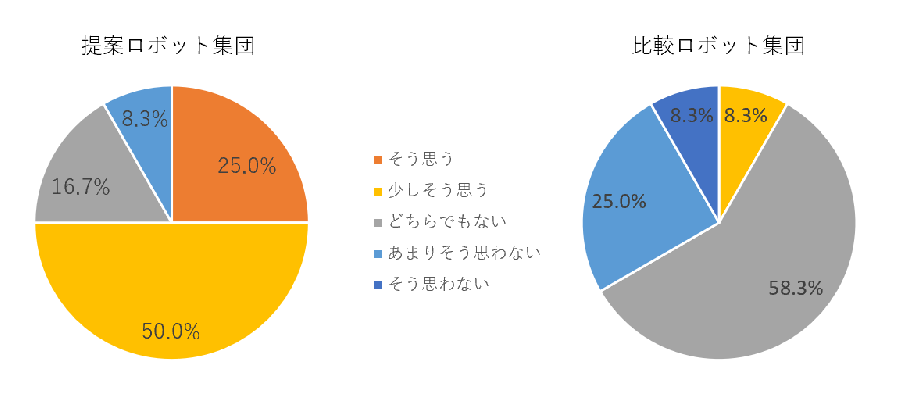
\includegraphics[width=15cm]{images/chapter4/Q1.eps}
  \caption{「ロボット集団との観戦を楽しむことができたか」のアンケート結果}
  \label{Q1}
 \end{center}
\end{figure}



\begin{figure}[!h]
 \begin{center}
\vspace{3cm}
  \centering
  \includegraphics[width=15cm]{images/chapter4/Q2.eps}
  \caption{「実際にロボット集団は観戦しているように感じたか」のアンケート結果}
  \label{Q2}
 \end{center}
\end{figure}



\newpage

\begin{figure}[!h]
 \begin{center}
\vspace{3cm}
  \centering
  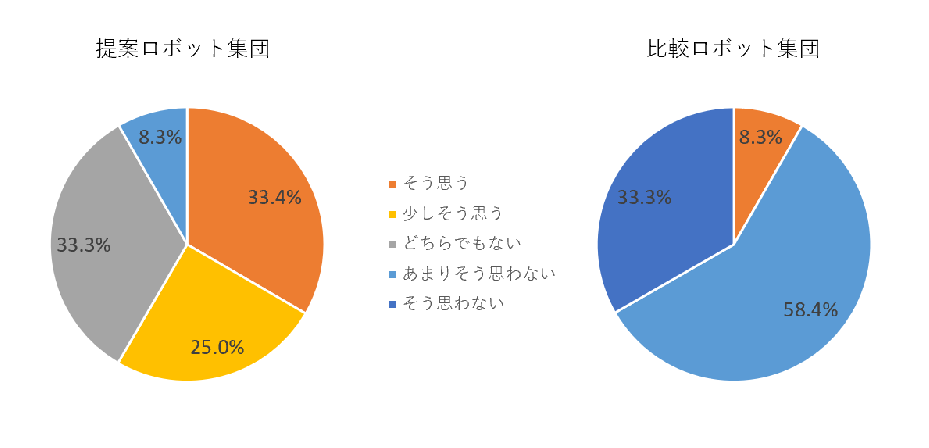
\includegraphics[width=15cm]{images/chapter4/Q3.eps}
  \caption{「ロボット集団との観戦で一体感を感じることができたか」のアンケート結果}
  \label{Q3}
 \end{center}
\end{figure}



\begin{figure}[!h]
 \begin{center}
\vspace{2cm}
  \centering
  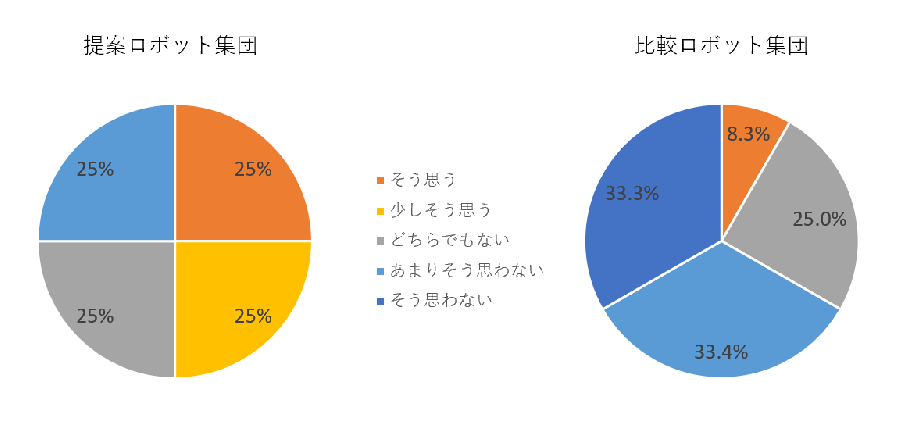
\includegraphics[width=15cm]{images/chapter4/Q4.eps}
  \caption{「ロボット集団との観戦で臨場感を感じることができたか」のアンケート結果}
  \label{Q4}
 \end{center}
\end{figure}

\newpage


\begin{figure}[!h]
 \begin{center}
\vspace{3cm}
  \centering
  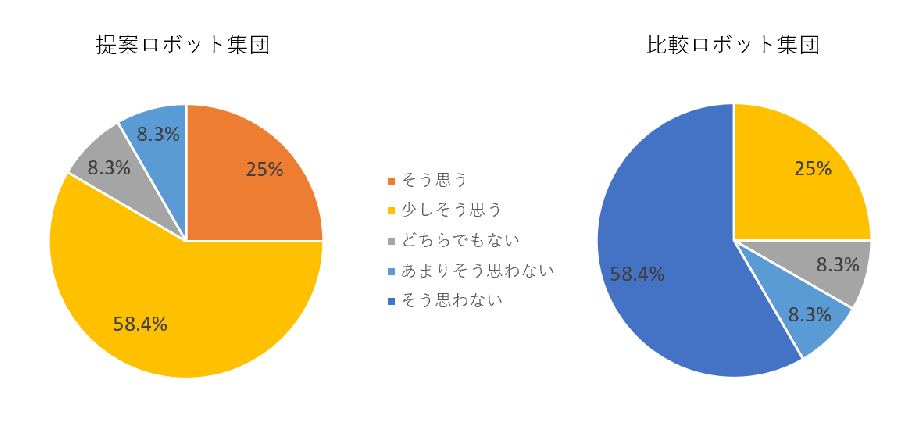
\includegraphics[width=15cm]{images/chapter4/Q5.eps}
  \caption{「ロボット集団の感情表出に感化されたか」のアンケート結果}
  \label{Q5}
 \end{center}
\end{figure}



\begin{figure}[!h]
 \begin{center}
\vspace{3cm}
  \centering
  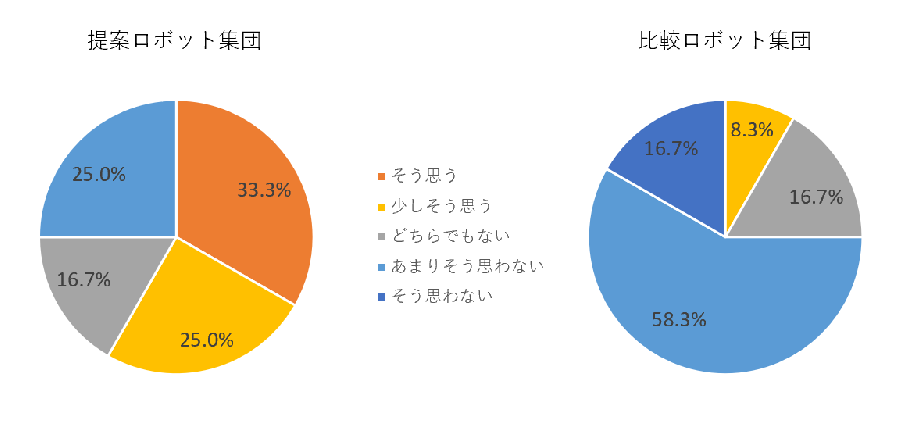
\includegraphics[width=15cm]{images/chapter4/Q6.eps}
  \caption{「ロボット集団に人間らしさを感じたか」のアンケート結果}
  \label{Q6}
 \end{center}
\end{figure}

\newpage



\begin{figure}[!h]
 \begin{center}
\vspace{3cm}
  \centering
  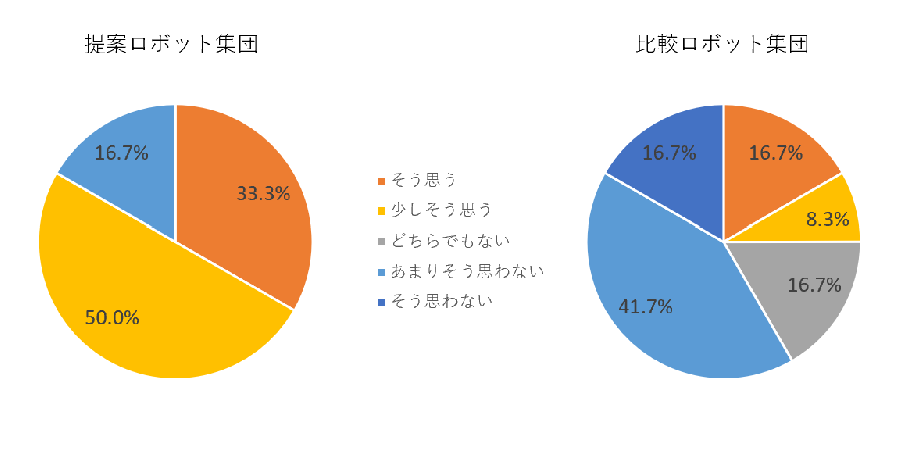
\includegraphics[width=15cm]{images/chapter4/Q7.eps}
  \caption{「ロボット集団に親しみを持てたか」のアンケート結果}
  \label{Q7}
 \end{center}
\end{figure}




\begin{figure}[!h]
 \begin{center}
\vspace{2cm}
  \centering
  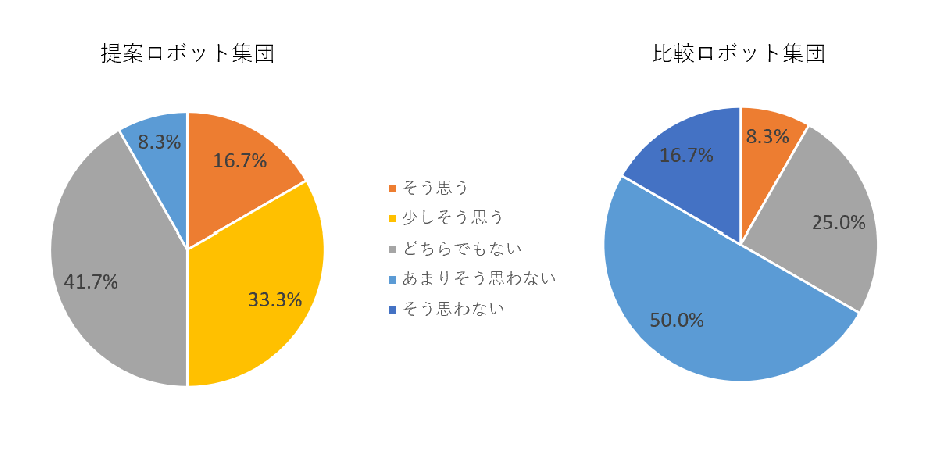
\includegraphics[width=15cm]{images/chapter4/Q8.eps}
  \caption{「またこのロボット集団と一緒に観戦したいか」のアンケート結果}
  \label{Q8}
 \end{center}
\end{figure}



\newpage

\vspace{1cm}
\begin{figure}[!h]
 \begin{center}
  \centering
  \includegraphics[width=15cm]{images/chapter4/Q9.eps}
  \caption{どちらのロボット集団の観戦が楽しかったか}
  \label{Q9}
 \end{center}
\end{figure}

\vspace{1cm}
\begin{figure}[!h]
 \begin{center}
  \centering
  \includegraphics[width=15cm]{images/chapter4/Q10.eps}
  \caption{どちらのロボット集団に一体感を感じたか}
  \label{Q10}
 \end{center}
\end{figure}

\newpage

\vspace{1cm}
\begin{figure}[!h]
 \begin{center}
  \centering
  \includegraphics[width=15cm]{images/chapter4/Q11.eps}
  \caption{どちらのロボット集団に臨場感を感じたか}
  \label{Q11}
 \end{center}
\end{figure}

\vspace{1cm}
\begin{figure}[!h]
 \begin{center}
  \centering
  \includegraphics[width=15cm]{images/chapter4/Q12.eps}
  \caption{どちらのロボット集団の感情表出に感化されたか}
  \label{Q12}
 \end{center}
\end{figure}

\newpage

\vspace{1cm}
\begin{figure}[!h]
 \begin{center}
  \centering
  \includegraphics[width=15cm]{images/chapter4/Q13.eps}
  \caption{どちらのロボット集団に人間らしさを感じたか}
  \label{Q13}
 \end{center}
\end{figure}

\vspace{1cm}
\begin{figure}[!h]
 \begin{center}
  \centering
  \includegraphics[width=15cm]{images/chapter4/Q14.eps}
  \caption{どちらのロボット集団に親しみを持てたか}
  \label{Q14}
 \end{center}
\end{figure}

\newpage

\vspace{1cm}
\begin{figure}[!h]
 \begin{center}
  \centering
  \includegraphics[width=15cm]{images/chapter4/Q15.eps}
  \caption{どちらのロボット集団とまた一緒に観戦したいか}
  \label{Q15}
 \end{center}
\end{figure}





\newpage

\section{考察}
\label{sec4.4}

図\ref{Q1}より,頻繁に感情を表出するロボット集団との観戦で,被験者は楽しさを感じていたことが分かる.これは,実空間での観戦を提案ロボット集団との観戦で再現できていたためだと考えられる.また,図\ref{Q2}~図\ref{Q5}より,被験者は提案ロボット集団との観戦で,本研究で示している臨場感の構成要素である,没入感や一体感,ロボット集団からの感情伝播に関する評価が高かったことが分かる.一方で,臨場感そのものについて問う質問では,半数の被験者がどちらでもない,あるいは低評価だと回答しており,十分な結果とは言えなかった.この結果から,没入感や一体感,感情伝播以外にも,スポーツ観戦において,臨場感を演出するために必要な要素があると考えられる.

両ロボットを比較する質問である図\ref{Q9}~図\ref{Q15}より,被験者の9割以上が,提案ロボット集団の方が,共に試合観戦を行うロボット集団に適していると感じていたことが分かる.この結果から,スポーツ観戦において臨場感を演出するためには,周囲の感情表出が必要不可欠であると考えられる.一方で,比較ロボット集団の方が適していると回答した被験者はほとんどいなかった.これは,本実験で設定したパラメータにより,提案ロボット集団と比較ロボット集団の感情表出のしやすさに差を付けすぎたことが原因であると考えられる.

また,自由記述で「ロボット集団が動作に合わせて歓声を挙げた方がいいと思った」「ロボット同士のハイタッチなどがあればより観戦していると感じることができると思った」などのロボットの感情表出に関する記述が多かった.一方で,「動作だけでも一体になっている感覚があった」という記述もあった.これらの記述から,観戦するロボットの動作による感情表出だけでも臨場感を演出することはできているが,感情表出の方法をより工夫することで,更なる臨場感の演出が期待できると考えられる.














